\documentclass[a4paper,10pt,titlepage]{jreport}

\usepackage{amsmath,amsfonts}
\usepackage{bm}
\usepackage[dvipdfmx]{graphicx}
\usepackage[dvipdfmx]{color}
\usepackage{here}
\usepackage{caption}
\usepackage{url}
\usepackage{listings}
\usepackage{longtable}

\lstset{
    basicstyle={\ttfamily},
    identifierstyle={\small},
    commentstyle={\small},
    keywordstyle={\small\bfseries},
    ndkeywordstyle={\small},
    stringstyle={\small\ttfamily},
    frame={tb},
    breaklines=true,
    columns=fixed,
    basewidth=0.465em,
    numbers=left,
    numberstyle={\scriptsize},
    lineskip=-0.5ex
}

\begin{document}

\title{One Touch Log プロセスについて}
\author{高橋龍馬, 中村優希}
\date{\today}
\maketitle

\section*{変更履歴}

\begin{longtable}[c]{|c|c|c|}
    \hline
        Ver. & 更新日 & 内容 \\
    \hline
    \endfirsthead
    \hline
        0.0.1 & 2024/06/26 & 叩き台作成 \\
    \hline
        0.1.0 & 2024/06/26 & イントロから戦略を追加 \\
    \hline
\end{longtable}

\newpage

\tableofcontents
\clearpage

\section{これについて} \label{sec:introduction}

\subsubsection{状況:}

当初開発を始めたサイクルにおいて、途中で何をすべきかわからなくなったため、新しいサイクルとして仕切り直すこととした。 \\
これまでの開発を第1サイクルとし、今後の開発を第2, 第3, ...サイクルとする。 \\
なお第2サイクルに入る前に、第1サイクルの事後分析を行い、プロジェクトとしての計画を立てるため、第1サイクルの戦略をする。 \\

現在までの状況と、今後どう進めるかは次のイメージ \\

\begin{figure}[H]
  \centering
  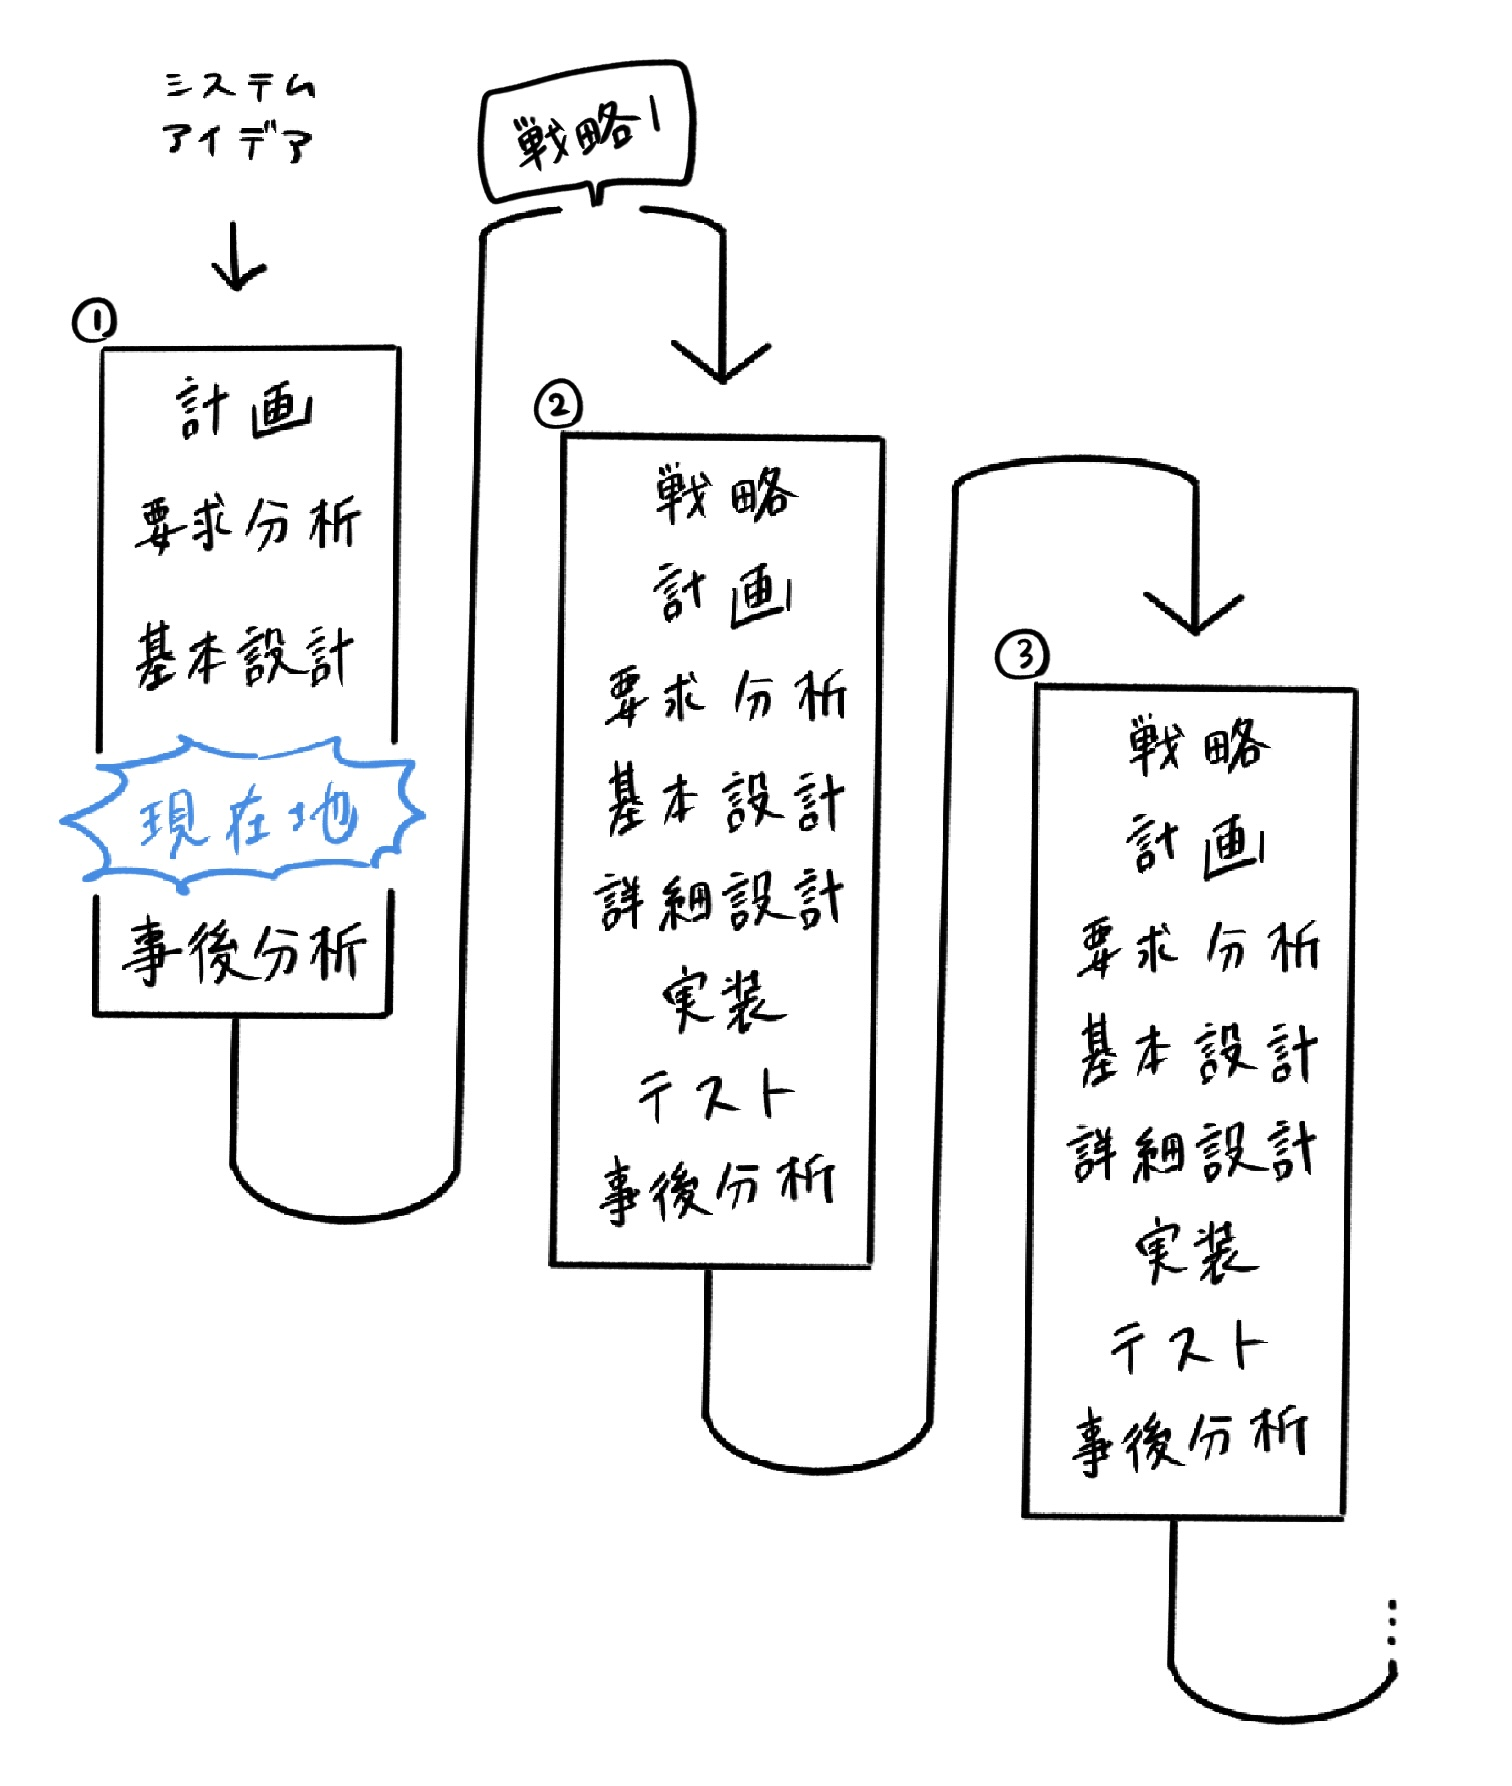
\includegraphics[width=80mm]{sections/cycle.jpg}
  \caption{サイクルの進め方}
  \label{fig:output}
\end{figure}

そこで、議事録という面を含むが、この文書で記述するのは次のとおり.

\begin{itemize}
  \item これまでの事後分析
  \item 本来すべきだった第1サイクルの戦略
  \begin{itemize}
    \item 概念設計
    \item 最終的にシステムが完成するまでの時間見積もり
    \item サイクル分割
  \end{itemize}
  \item これからのサイクルの進め方
\end{itemize}


\section{第2サイクルに入る前の整理} \label{sec:arrangement}

ここは議事録のようなもの.

\subsection{第1サイクルの事後分析について}

これまで作成した成果物は次のとおり.

\begin{itemize}
  \item 概念設計
  \item 背景と目的
  \item 用語定義
  \item 要件定義
  \item データ要件(ログ)
  \item 技術要件
  \item アプリ形態(クロスプロットフォーム)
  \item アーキテクチャ図
  \item 画面設計
  \item 機能のシーケンス図
\end{itemize}

計画〜基本設計のフェーズに当てはめると、次のようになる.なお内容が不十分だと思われるものには「?」をつけた.

\begin{table}[htbp]
  \centering
  \begin{tabular}{|l|l|}
  \hline
    計画 &
    \begin{tabular}{l}
    概念設計 \\
    \end{tabular} \\
  \hline
    要求定義 &
    \begin{tabular}{l}
      背景と目的(?) \\
      \quad •ゼミで指摘されたため内容不十分の可能性あり \\
      \quad •レポートで表示するグラフが適切かどうか \\
      用語定義(?) \\
      \quad •初期に作成したので内容不十分の可能性あり \\
      要件定義 \\
      データ要件(ログ) \\
      技術要件 \\
      アプリ形態(クロスプロットフォーム) \\
      \end{tabular} \\
  \hline
    基本設計 &
    \begin{tabular}{l}
      アーキテクチャ図 \\
      画面設計(?) \\
      機能のシーケンス図 \\
      \end{tabular} \\
  \hline
  \end{tabular}
\end{table}

事後分析は以上とする.

% 構成管理計画

\subsection{第1サイクルの戦略について}

\subsubsection{概念設計}

現時点で考えられる機能は次のとおり. なお要求と並べているのは、要求を満たす機能であるかどうかを確認するため.

\begin{table}[htbp]
  \centering
  \begin{tabular}{|l|l|}
  \hline
    要求 & 機能 \\
  \hline

  \hline
    ログを取りたい &
    \begin{tabular}{l}
      ログを計測する画面 \\
      \quad •開始時刻を取得 \\
      \quad •終了時刻を取得 \\
      \quad •ログ情報を取得し、保存 \\
      ログを編集する機能 \\
      \quad •更新されたログ情報を保存 \\
      ログを削除する機能 \\
      \quad •指定されたログを削除
      ユーザーごとにログを識別する機能 \\
      \quad •サインアップ \\
      \quad •サインイン \\
      \quad •ユーザー情報の編集 \\
    \end{tabular} \\
  \hline
    ログを閲覧したい &
    \begin{tabular}{l}
      デイリーレポートを表示する画面 \\
      \quad •日付を指定し、その日のログを表示 \\
      \quad •その日の統計情報を表示 \\
      \quad •その日のログについてのグラフを表示 \\
      週間レポートを表示する画面 \\
      \quad •週を指定し、その週のログを表示 \\
      \quad •その週の統計情報を表示 \\
      \quad •その週のログについてのグラフを表示 \\
      月間レポートを表示する画面 \\
      \quad •月を指定し、その月のログを表示 \\
      \quad •その月の統計情報を表示 \\
      \quad •その月のログについてのグラフを表示 \\
      エクスポート機能 \\
      \quad •各レポートからデータをエクスポート \\
    \end{tabular} \\
  \hline
    ログをとる習慣をつけたい &
    \begin{tabular}{l}
      リマインド機能 \\
      \quad •ログ計測の開始リマインドを送信 \\
      \quad •ログ計測の終了リマインドを送信 \\
      \quad •リマインドの設定 \\
    \end{tabular} \\
  \hline
  \end{tabular}
\end{table}

表から、画面と機能を整理すると次のようになる.

\begin{table}[H]
  \centering
  \caption{機能}
  \begin{tabular}{|l|l|}
  \hline
    機能 & LOC \\
  \hline

  \hline
    開始時刻を取得 & 30 + 0 = 30 \\
  \hline
    終了時刻を取得 & 30 + 0 = 30 \\
  \hline
    ログ情報を取得し、保存 & 120 + 20 = 140 \\
  \hline
    更新されたログ情報を保存 & 60 + 50 = 110 \\
  \hline
    指定されたログを削除 & 60 + 50 = 110 \\
  \hline

  \hline
    ある期間を指定し、その期間のログを表示 & 20 + 50 = 70 \\
  \hline
    ある期間の統計情報を表示 & 40 + 20 = 60 \\
  \hline
    ある期間のログについてのグラフを表示 & 100 + 0 = 100 \\
  \hline
    各レポートからデータをエクスポート & 40 + 0 = 40 \\
  \hline

  \hline
    ログ計測の開始リマインドを送信 & 20 + 0 = 20 \\
  \hline
    ログ計測の終了リマインドを送信 & 20 + 0 = 20 \\
  \hline
    リマインドの設定 & 250 + 50 = 300 \\
  \hline

  \hline
    サインアップ &  90 + 30 = 120 \\
  \hline
    サインイン & 90 + 30 = 120 \\
  \hline
    ユーザー情報の編集 & 100 + 40 = 140 \\
  \hline
  \end{tabular}
\end{table}

\begin{table}[H]
  \centering
  \caption{想定画面}
  \begin{tabular}{|l|}
  \hline
    サインアップ画面  \\
    サインイン画面 \\
    計測開始画面 \\
    計測中画面 \\
    計測終了画面 \\
    設定画面 \\
    デイリーレポート画面 \\
    週間レポート画面 \\
    月間レポート画面 \\
  \hline
  \end{tabular}
\end{table}

バックエンド
フロントエンド機能
UI


\subsubsection{時間見積もり}

想定画面について、1画面あたり2時間とすると、デザインにかかる時間は $9 * 12 = 108$ 時間

また、チーム 2 LOC/hour で開発できると仮定すると、上記の機能は次のような時間がかかる.

\begin{table}[H]
  \centering
  \caption{機能}
  \begin{tabular}{|l|l|}
  \hline
    機能 & 時間見積もり(h) \\
  \hline

  \hline
    開始時刻を取得 & 10 \\
  \hline
    終了時刻を取得 & 10 \\
  \hline
    ログ情報を取得し、保存 & 46.6 \\
  \hline
    更新されたログ情報を保存 & 36.6 \\
  \hline
    指定されたログを削除 & 36.6 \\
  \hline

  \hline
    ある期間を指定し、その期間のログを表示 & 13.3 \\
  \hline
    ある期間の統計情報を表示 & 20 \\
  \hline
    ある期間のログについてのグラフを表示 & 33.3 \\
  \hline
    各レポートからデータをエクスポート & 13.3 \\
  \hline

  \hline
    ログ計測の開始リマインドを送信 & 6.6 \\
  \hline
    ログ計測の終了リマインドを送信 & 6.6 \\
  \hline
    リマインドの設定 & 100 \\
  \hline

  \hline
    サインアップ & 40 \\
  \hline
    サインイン & 40 \\
  \hline
    ユーザー情報の編集 & 46.6 \\
  \hline
  \end{tabular}
\end{table}

よって、プロジェクトの時間見積もりは $108 + 459.5 = 567.5$ 時間となる.

1人あたりの1週間の平均作業時間が14時間のため、プロジェクトの期間は $567.5 / (14 * 2) = 20.3$ 週となる. \\

すなわち、約4.8ヶ月弱ほどかかると見積もられる.


\subsubsection{サイクル分割}

当初設定したサイクル分割は次のとおりであった.

\begin{table}[H]
  \centering
  \begin{tabular}{|l|l|}
  \hline
    第1サイクル &
    \begin{tabular}{l}
      ログを計測する機能 \\
      ログを編集・削除する機能 \\
      デイリーレポートを表示する機能 \\
      リマインド機能 \\
      サインアップ・サインイン
    \end{tabular} \\
  \hline
    第2サイクル &
    \begin{tabular}{l}
      週間レポートを表示する機能 \\
      月間レポートを表示する機能 \\
      エクスポート機能
    \end{tabular} \\
  \hline
    第3サイクル &
    \begin{tabular}{l}
      ユーザー情報の編集機能 \\
      カテゴリのレコメンド機能
    \end{tabular} \\
  \hline
    第4サイクル &
    \begin{tabular}{l}
      ユーザー情報の公開機能 \\
    \end{tabular} \\
  \hline
  \end{tabular}
\end{table}

時間見積もりを参考に、サイクル分割を見直す.

\begin{table}[H]
  \centering
  \begin{tabular}{|l|l|l|}
  \hline
    サイクル & 機能 & かかる時間(h) \\
  \hline

  \hline
    第1サイクル &
    \begin{tabular}{l}
      開始時刻を取得 \\
      終了時刻を取得 \\
      ログ情報を取得し、保存 \\
    \end{tabular} &
    66.6 \\
  \hline
    第2サイクル &
    \begin{tabular}{l}
      ある期間を指定し、その期間のログを表示 \\
      ある期間の統計情報を表示 \\
      ある期間のログについてのグラフを表示 \\
    \end{tabular} &
    66.6 \\
  \hline
    第3サイクル &
    \begin{tabular}{l}
      更新されたログ情報を保存 \\
      指定されたログを削除 \\
    \end{tabular} &
    73.2 \\
  \hline
    第4サイクル &
    \begin{tabular}{l}
      リマインドの設定
    \end{tabular} &
    100 \\
  \hline
    第5サイクル &
    \begin{tabular}{l}
      ログ計測の開始リマインドを送信 \\
      ログ計測の終了リマインドを送信 \\
    \end{tabular} &
    13.2 \\
  \hline
    第6サイクル &
    \begin{tabular}{l}
      サインアップ \\
      サインイン \\
    \end{tabular} &
    80 \\
  \hline
    第7サイクル &
    \begin{tabular}{l}
      ユーザー情報の編集 \\
      各レポートからデータをエクスポート \\
    \end{tabular} &
    59.9 \\
  \hline
  \end{tabular}
\end{table}



\section{各サイクルの進め方} \label{sec:process}

2回目以降のサイクルで行うことを示す. \\

\begin{longtable}[l]{|p{1.5cm}|p{11cm}|}
  \endfirsthead
  \hline
    目的 & 2回目以降のサイクルにおける機能の開発をガイドする \\
  \hline
    事前条件 &
    \begin{tabular}{l}
      前回のサイクルでの成果物
    \end{tabular} \\
  \hline
  \hline
    戦略 &
    \begin{tabular}{l}
      前回のサイクルで作成した成果物を確認する. \\
      今回のサイクルで行うことを定義する. \\
    \end{tabular} \\
  \hline
    計画 &
    \begin{tabular}{l}
      規模見積もりをする. \\
      \quad •WBS \\
      規模見積もりから, 時間見積もりをする. \\
      スケジュールを作成する. \\
      \quad •ms project \\
    \end{tabular} \\
  \hline
    要求分析 &
    \begin{tabular}{l}
      なんのためにどんなものを作りたいのかを定義する \\
      \quad •システム化の背景 \\
      \quad •システムの目的 \\
      利用者がシステムで行うことを定義する. \\
      \quad •システムの全体像 \\
      \quad •ユースケース \\
      実現したいものを整理・分析する. \\
      \quad •要求一覧 \\

      要求に関する画面の要件を作成する \\
      \quad •画面要件 \\
      画面の操作や機能を定義する \\
      \quad •機能要件 \\
      \quad •非機能要件 \\
      データ要件を定義する \\
      \quad •データ要件 \\
      システムテスト計画を作成する \\
      \quad •機能テスト \\
      \quad •シナリオテスト \\
    \end{tabular} \\
  \hline
    基本設計 &
    \begin{tabular}{l}
      基本設計書のフォーマット作成 \\
      アーキテクチャ設計の作成 \\
      モジュール設計の作成 \\
      \quad •基本設計書 \\
      統合テスト計画の作成
    \end{tabular} \\
  \hline
    詳細設計 &
    \begin{tabular}{l}
      詳細設計書のフォーマット作成 \\
      詳細設計の作成 \\
      \quad •詳細設計書 \\
      単体テスト計画の作成
    \end{tabular} \\
  \hline
    実装 &
    \begin{tabular}{l}
      詳細設計書に基づいて実装 \\
    \end{tabular} \\
  \hline
    テスト &
    \begin{tabular}{l}
      単体テストを行う \\
      結合テストを行う \\
      システムテストを行う \\
    \end{tabular} \\
  \hline
    事後分析 &
    \begin{tabular}{l}
      今回作成した成果物を分析する \\
      作成するべき事柄が判明したら, 次回のサイクルのために記録する \\
    \end{tabular} \\
  \hline
\end{longtable}


\end{document}
